\documentclass[11pt,aspectratio=169]{beamer}

\usetheme{Madrid}
\usecolortheme{seahorse}

\usepackage[utf8]{inputenc}
\usepackage{amsmath,amssymb}
\usepackage{algpseudocode}
\usepackage{algorithmicx}
\usepackage{xcolor}
\usepackage{listings}
\usepackage{booktabs}
\usepackage{tikz}
\usetikzlibrary{arrows.meta,positioning,fit,backgrounds}

\setbeamertemplate{navigation symbols}{}
\setbeamertemplate{footline}[frame number]

\lstdefinestyle{py}{
  language=Python,
  basicstyle=\ttfamily\scriptsize,
  keywordstyle=\color{blue!70!black}\bfseries,
  commentstyle=\color{gray},
  stringstyle=\color{green!40!black},
  showstringspaces=false,
  breaklines=true,
  numbers=left,
  numberstyle=\tiny\color{gray},
  frame=single,
  xleftmargin=1.5em,
  aboveskip=0.3em,
  belowskip=0.3em
}

\title{LeetCode Deep Dive}
\subtitle{From First Instinct to Optimal Algorithm: Backtracking on NP-Hard Search Spaces\\
\small Week 12 Supplement -- TOAE209/TOAH209: Design and Analysis of Algorithms}
\author{Foreign Trade University}
\date{}

\begin{document}

% ---------------------------------------------------------------
\begin{frame}
  \titlepage
\end{frame}
% ---------------------------------------------------------------

\begin{frame}{Outline}
  \tableofcontents
\end{frame}

% =================================================================
\section{A Framework for Attacking a Search Problem}
% =================================================================

\begin{frame}{Why walk through LeetCode problems?}
  \begin{itemize}
    \item This week's \texttt{LEETCODE.md} list gives ten Week 12 problems to
    \emph{practice on your own}. This deck narrates the thinking process for two of
    them end to end, so you can reuse the process on the rest.
    \item We pick one \textcolor{blue!50!black}{\textbf{Medium}} (\emph{Combination
    Sum}) and one \textcolor{red!60!black}{\textbf{Hard}} (\emph{N-Queens}) --
    both are exactly the kind of \textbf{exponential search} problem this week's
    lecture explains \emph{why} no polynomial algorithm is known for the general case.
    \item Combination Sum is literally the ``find a certificate'' version of
    \textsc{Subset Sum} (with repetition allowed) -- a problem this week's lecture
    notes prove is NP-complete. That is \emph{why} we reach for backtracking instead of
    a clean polynomial recipe.
  \end{itemize}
\end{frame}

\begin{frame}{The four-step process we will repeat twice}
  \begin{enumerate}
    \item \textbf{First instinct.} The algorithm that follows most directly from
    re-reading the problem: generate every candidate, then filter.
    \item \textbf{Measure why it hurts.} Plug the problem's real constraints into the
    brute-force bound and watch it explode.
    \item \textbf{Find the structural insight.} What lets you \textbf{prune} a branch
    the instant it cannot lead anywhere, instead of finishing it and checking at the
    end?
    \item \textbf{Implement it}, verify a hand trace, then look for the
    \emph{programming-level} tricks that make the implementation itself fast.
  \end{enumerate}
  \begin{alertblock}{This mirrors the course}
    NP-completeness does not mean ``give up.'' It means: stop looking for a polynomial
    exact algorithm, and instead make the exponential search as small as the
    \emph{instance} allows -- exactly what backtracking with pruning does.
  \end{alertblock}
\end{frame}

% =================================================================
\section{Problem 1 (Medium): Combination Sum}
% =================================================================

\begin{frame}{Problem statement}
  \begin{block}{LeetCode 39 -- Combination Sum (\textcolor{blue!50!black}{Medium})}
    Given an array of \textbf{distinct} positive integers \texttt{candidates} and a
    target integer \texttt{target}, return all unique combinations of
    \texttt{candidates} that sum to \texttt{target}. The \textbf{same} number may be
    chosen an unlimited number of times.
  \end{block}
  \begin{itemize}
    \item Constraints (LeetCode): $1 \le$ \texttt{candidates.length} $\le 30$,
    $1 \le$ \texttt{candidates[i]} $\le 40$ (all distinct), $1 \le$ \texttt{target}
    $\le 40$.
    \item This is \textsc{Subset Sum with repetition}: this week's lecture proves
    (general) \textsc{Subset Sum} is NP-complete -- so no polynomial algorithm is
    expected for the worst case, and we should not be surprised the best known approach
    is exponential search, done \emph{smartly}.
  \end{itemize}
\end{frame}

\begin{frame}{Worked example}
  \texttt{candidates = [2,3,6,7]}, \texttt{target = 7}
  \begin{itemize}
    \item $2+2+3 = 7$ and $7 = 7$ are the only two ways to reach the target using
    (possibly repeated) candidates.
    \item \textbf{Answer:} \texttt{[[2,2,3],[7]]}.
    \item Note what is \emph{not} allowed: $[2,2,3]$ and $[2,3,2]$ count as the
    \textbf{same} combination (order doesn't matter) -- the algorithm must avoid
    reporting both.
  \end{itemize}
\end{frame}

\begin{frame}{First instinct: generate, then filter}
  \begin{block}{Most direct reading of the problem}
    ``Find every multiset of candidates summing to target'' $\Rightarrow$ enumerate
    every sequence of candidates (with repetition, up to the depth where the sum could
    still reach \texttt{target}), sum each one, keep the ones that hit exactly
    \texttt{target}, then deduplicate permutations of the same multiset.
  \end{block}
  \begin{algorithmic}[1]
    \For{every sequence $(c_1, c_2, \dots, c_d)$ of candidates, $d = 1$ to
    $\lceil \text{target} / \min(\text{candidates}) \rceil$}
      \If{$\sum c_i = \text{target}$} remember $\text{sorted}(c_1,\dots,c_d)$ \EndIf
    \EndFor
    \State deduplicate the remembered multisets
  \end{algorithmic}
\end{frame}

\begin{frame}{Why this is bad}
  \begin{itemize}
    \item With up to $30$ distinct candidates and a search depth of up to $40$ (target
    $\le 40$, candidate values $\ge 1$), the number of raw sequences is up to
    $30^{40}$ -- astronomically larger than anything checkable.
    \item Even generously assuming small candidate values keep the depth shallow, this
    approach explores \textbf{every} sequence, including ones that already exceed
    \texttt{target} after the very first pick, before ever checking the sum.
    \item It also does needless work \emph{after} the fact: generating both
    $[2,2,3]$ and $[2,3,2]$ and $[3,2,2]$ and then discovering they are duplicates.
  \end{itemize}
  \begin{alertblock}{The smell to notice}
    ``Generate everything, then filter/deduplicate'' is almost always a sign that a
    huge fraction of the generated work was doomed from a much earlier point --
    exactly what pruning is for.
  \end{alertblock}
\end{frame}

\begin{frame}{The structural insight}
  \begin{itemize}
    \item \textbf{Prune as soon as a partial sum cannot possibly work.} If the running
    remainder drops below $0$, stop that branch immediately -- no need to finish
    building the sequence.
    \item \textbf{Sort the candidates once, and only try candidates from the current
    index onward.} Requiring the next pick's index to be $\ge$ the current one
    (instead of $\ge 0$) makes $[2,2,3]$ reachable but $[2,3,2]$ and $[3,2,2]$
    \emph{unreachable in the first place} -- no deduplication step needed at all.
    \item \textbf{Sorted candidates let you \texttt{break} the loop early}, not just
    \texttt{continue}: once one candidate exceeds the remaining target, every later
    (larger) candidate does too.
  \end{itemize}
\end{frame}

\begin{frame}{Optimal algorithm: pseudocode}
  \footnotesize
  \begin{algorithmic}[1]
    \Function{CombinationSum}{candidates, target}
      \State sort candidates ascending
      \State $path \gets []$;\ $results \gets []$
      \State \Call{Backtrack}{$0$, target}
      \State \Return $results$
    \EndFunction
    \Function{Backtrack}{start, remain}
      \If{$remain = 0$} record a copy of $path$ into $results$;\ \Return \EndIf
      \For{$i \gets start$ \textbf{to} $\text{len(candidates)} - 1$}
        \If{$candidates[i] > remain$} \textbf{break} \Comment{sorted: all later are bigger too}\EndIf
        \State append $candidates[i]$ to $path$
        \State \Call{Backtrack}{$i$, $remain - candidates[i]$} \Comment{$i$, not $i+1$: reuse allowed}
        \State remove last element of $path$
      \EndFor
    \EndFunction
  \end{algorithmic}
\end{frame}

\begin{frame}[fragile]{Hand-verified trace on the worked example}
  \begin{lstlisting}[style=py,numbers=none,aboveskip=0pt,belowskip=0pt]
backtrack(start=0, remain=7, path=[])
  try 2 -> path=[2],   remain=5
    try 2 -> path=[2,2], remain=3
      try 2 -> path=[2,2,2], remain=1
        try 2 -> 2 > remain(1): break
      try 3 -> path=[2,2,3], remain=0  ==> RECORD [2,2,3]
      try 6 -> 6 > remain(3): break
    try 3 -> path=[2,3], remain=2
      try 3 -> 3 > remain(2): break
    try 6 -> 6 > remain(5): break
  try 3 -> path=[3],   remain=4
    try 3 -> path=[3,3], remain=1
      try 3 -> 3 > remain(1): break
    try 6 -> 6 > remain(4): break
  try 6 -> path=[6],   remain=1
    try 6 -> 6 > remain(1): break
  try 7 -> path=[7],   remain=0  ==> RECORD [7]

result: [[2,2,3],[7]]      (16 candidate-tries total)
  \end{lstlisting}
\end{frame}

\begin{frame}{Complexity: how much does pruning actually save?}
  \small
  These are \textbf{real, measured} node counts (not estimates) for the pruned
  backtracking search:
  \begin{center}
  \begin{tabular}{@{}lrr@{}}
    \toprule
    Instance & Candidate-tries \emph{without} early \texttt{break} & \emph{with} it \\
    \midrule
    \texttt{[2,3,6,7]}, target $7$ & $27$ & $16$ \\
    $15$ candidates ($1..15$), target $40$ & $1{,}018{,}761$ & $327{,}704$ \\
    \bottomrule
  \end{tabular}
  \end{center}
  \begin{itemize}
    \item Both columns already prune on $remain < 0$ -- sorting plus an early
    \texttt{break} (instead of \texttt{continue}) is a \emph{free} extra $\sim 3\times$
    reduction in explored nodes on the stress case above.
    \item Worst case is still exponential (this is NP-hard!) -- but ``exponential''
    and ``$327{,}704$ nodes in milliseconds'' can both be true at once.
  \end{itemize}
\end{frame}

\begin{frame}[fragile]{Python implementation}
  \begin{lstlisting}[style=py,aboveskip=0pt,belowskip=0pt]
def combinationSum(candidates, target):
    candidates.sort()
    results = []
    path = []

    def backtrack(start, remain):
        if remain == 0:
            results.append(path.copy())   # snapshot -- path keeps mutating after this
            return
        for i in range(start, len(candidates)):
            if candidates[i] > remain:
                break                      # sorted, so every later i is worse too
            path.append(candidates[i])
            backtrack(i, remain - candidates[i])   # i, not i + 1: reuse allowed
            path.pop()

    backtrack(0, target)
    return results
  \end{lstlisting}
\end{frame}

\begin{frame}{Implementation tips \& tricks (the programming side)}
  \small
  \begin{itemize}
    \item \textbf{\texttt{path.copy()}, never \texttt{path}.} \texttt{path} is one
    mutable list reused across the whole recursion; appending a \emph{reference} to it
    in \texttt{results} means every later \texttt{append}/\texttt{pop} silently
    corrupts every previously recorded answer. This is one of the most common real bugs
    in backtracking code.
    \item \textbf{Sort once, outside the recursion.} Sorting inside \texttt{backtrack}
    (or on every call) would cost $O(n \log n)$ per node instead of once total --
    a correctness-preserving but performance-destroying mistake.
    \item \textbf{\texttt{append}/\texttt{pop} instead of list concatenation.}
    \texttt{path + [c]} allocates a new list at \emph{every} node; \texttt{path.append};
    \texttt{...}; \texttt{path.pop()} mutates in place and is the standard backtracking
    idiom for exactly this reason.
  \end{itemize}
\end{frame}

% =================================================================
\section{Problem 2 (Hard): N-Queens}
% =================================================================

\begin{frame}{Problem statement}
  \begin{block}{LeetCode 51 -- N-Queens (\textcolor{red!60!black}{Hard})}
    Place $n$ queens on an $n \times n$ chessboard so that no two queens attack each
    other (share a row, column, or diagonal). Return \textbf{all} distinct solutions.
  \end{block}
  \begin{itemize}
    \item Constraints (LeetCode): $1 \le n \le 9$.
    \item This is the canonical constraint-satisfaction search problem, and (like
    Graph Coloring, proved NP-complete this week) it belongs to the same family: an
    exponential number of candidate placements, checked against \emph{local}
    pairwise constraints.
  \end{itemize}
\end{frame}

\begin{frame}{Worked example: one solution for $n=4$}
  \begin{columns}
  \begin{column}{0.4\textwidth}
  \begin{center}
  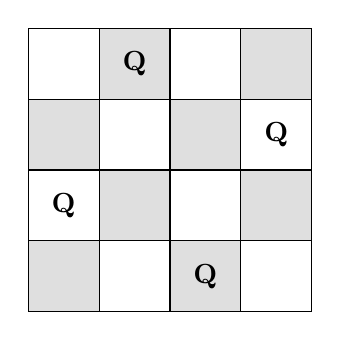
\begin{tikzpicture}[scale=0.9]
    \foreach \x in {0,...,3} {
      \foreach \y in {0,...,3} {
        \pgfmathtruncatemacro{\shade}{Mod(\x+\y,2)}
        \ifnum\shade=0
          \fill[gray!25] (\x,\y) rectangle (\x+1,\y+1);
        \fi
      }
    }
    \draw[step=1cm,black] (0,0) grid (4,4);
    \node at (1.5,3.5) {\textbf{Q}};
    \node at (3.5,2.5) {\textbf{Q}};
    \node at (0.5,1.5) {\textbf{Q}};
    \node at (2.5,0.5) {\textbf{Q}};
  \end{tikzpicture}
  \end{center}
  \end{column}
  \begin{column}{0.6\textwidth}
  \small
  Queens at row,col $(0,1), (1,3), (2,0), (3,2)$ (rows top to bottom).
  \begin{itemize}
    \item No two share a row (one queen per row, by construction) or column
    ($1,3,0,2$ are all distinct).
    \item No two share a diagonal: every $|\Delta\text{row}| \ne |\Delta\text{col}|$
    pair -- check e.g.\ $(0,1)$ vs.\ $(3,2)$: $\Delta\text{row}=3$,
    $\Delta\text{col}=1$, not equal, safe.
    \item $n=4$ has exactly \textbf{2} solutions total (this one and its mirror
    image).
  \end{itemize}
  \end{column}
  \end{columns}
\end{frame}

\begin{frame}{First instinct: generate every placement, then check}
  \begin{block}{Most direct reading of the problem}
    ``Try every way to place $n$ queens, keep the valid ones'' $\Rightarrow$ since one
    queen per row is clearly required (two queens can never share a row), try every
    choice of column for every row independently, then check the \emph{whole} board
    for conflicts.
  \end{block}
  \begin{algorithmic}[1]
    \For{every function $f: \{0,\dots,n-1\} \to \{0,\dots,n-1\}$} \Comment{$n^n$ of them}
      \State place queen at $(row, f(row))$ for each row
      \If{no two queens attack each other} \Comment{$O(n^2)$ check}
        \State record this board
      \EndIf
    \EndFor
  \end{algorithmic}
\end{frame}

\begin{frame}{Why this is bad}
  \small
  These are \textbf{real, measured} numbers, not estimates (computed directly for
  this deck):
  \begin{center}
  \begin{tabular}{@{}lr@{}}
    \toprule
    Quantity (at $n=8$) & Value \\
    \midrule
    Column-assignments to generate ($n^n$) & $16{,}777{,}216$ \\
    Elementary ops incl.\ $O(n^2)$ validity check per board & $\approx 1{,}073{,}741{,}824$ \\
    \textbf{Actual number of solutions} & $\mathbf{92}$ \\
    \bottomrule
  \end{tabular}
  \end{center}
  \begin{itemize}
    \item Over a \textbf{billion} elementary operations to find $92$ valid boards --
    and every invalid board is only discovered \emph{after} being fully built.
  \end{itemize}
  \begin{alertblock}{The smell to notice (again)}
    ``Build the whole candidate, then check it'' -- the same pattern as Combination
    Sum's naive approach. The fix is the same idea too: check \emph{while} building, and
    stop the instant a partial choice is already invalid.
  \end{alertblock}
\end{frame}

\begin{frame}{The structural insight}
  \begin{itemize}
    \item Row-by-row placement already lets you check for conflicts \textbf{as you
    go}: when you are about to place row $r$'s queen, it can only conflict with the
    $r$ queens already placed in rows $0, \dots, r-1$ -- rows $>r$ don't exist yet.
    \item So the moment column $c$ conflicts with an already-placed queen (same
    column, or same diagonal), \textbf{skip it immediately} -- never recurse into a
    board that is already broken.
    \item This turns the search from ``generate $n^n$ complete boards, then filter''
    into ``explore only the prefixes that were valid at every step so far'' -- and an
    invalid prefix of length $k$ prunes away all $n^{n-k}$ boards that would have
    extended it.
  \end{itemize}
\end{frame}

\begin{frame}{Optimal algorithm: pseudocode}
  \footnotesize
  \begin{algorithmic}[1]
    \Function{Solve}{$n$}
      \State $cols \gets \emptyset$;\ $diag_1 \gets \emptyset$;\ $diag_2 \gets \emptyset$
      \Comment{sets of used columns / diagonals}
      \State \Call{Place}{$0$}
    \EndFunction
    \Function{Place}{row}
      \If{$row = n$} record current board;\ \Return \EndIf
      \For{$c \gets 0$ \textbf{to} $n-1$}
        \If{$c \in cols$ \textbf{or} $(row-c) \in diag_1$ \textbf{or} $(row+c) \in diag_2$}
          \State \textbf{continue} \Comment{conflict -- skip, don't even recurse}
        \EndIf
        \State add $c, row{-}c, row{+}c$ to $cols, diag_1, diag_2$
        \State \Call{Place}{$row+1$}
        \State remove $c, row{-}c, row{+}c$ from $cols, diag_1, diag_2$
      \EndFor
    \EndFunction
  \end{algorithmic}
\end{frame}

\begin{frame}{Hand-verified trace for $n=4$}
  \scriptsize
  \begin{center}
  \begin{tabular}{@{}c p{4.6cm} p{5.4cm}@{}}
    \toprule
    step & action & remark \\
    \midrule
    1 & row0: try col0 & placed $(0,0)$ \\
    2 & row1: cols $0,1$ attacked; try col2 & placed $(1,2)$ \\
    3 & row2: cols $0,1,2,3$ all attacked & dead end -- backtrack \\
    4 & row1: try col3 (last option) & placed $(1,3)$ \\
    5 & row2: only col1 free & placed $(2,1)$ \\
    6 & row3: cols $0,1,2,3$ all attacked & dead end -- backtrack all the way past row0=0 \\
    7 & row0: try col1 & placed $(0,1)$ \\
    8 & row1: only col3 free & placed $(1,3)$ \\
    9 & row2: only col0 free & placed $(2,0)$ \\
    10 & row3: only col2 free & \textbf{valid! solution} $(0,1),(1,3),(2,0),(3,2)$ \\
    \bottomrule
  \end{tabular}
  \end{center}
  Matches the diagram two slides ago exactly. (The search continues afterward to find
  the second, mirror-image solution.)
\end{frame}

\begin{frame}{Complexity: naive vs.\ pruned, at $n=8$}
  \small
  Also real, measured node counts:
  \begin{center}
  \begin{tabular}{@{}lr@{}}
    \toprule
    Approach & Nodes / boards touched \\
    \midrule
    Generate all $n^n$ boards, then check ($O(n^2)$ each) & $\approx 1.07 \times 10^{9}$
    elementary ops \\
    \textbf{Backtrack, check while placing} & $\mathbf{15{,}720}$ candidate-tries \\
    \bottomrule
  \end{tabular}
  \end{center}
  \begin{itemize}
    \item That is roughly a $68{,}000\times$ reduction in work for the \emph{same}
    correct answer (all $92$ solutions).
    \item Still exponential in the worst case -- this is exactly the ``theory vs.\
    practice'' gap this week's supplement deck discusses for SAT solvers.
  \end{itemize}
\end{frame}

\begin{frame}[fragile]{Python implementation (part 1: the search)}
  \begin{lstlisting}[style=py,aboveskip=0pt,belowskip=0pt]
def solveNQueens(n):
    results = []
    board = []                 # board[row] = column of that row's queen
    cols, diag1, diag2 = set(), set(), set()

    def place(row):
        if row == n:
            results.append(render(board, n))
            return
        for c in range(n):
            if c in cols or (row - c) in diag1 or (row + c) in diag2:
                continue                          # conflict: skip, don't recurse
            cols.add(c); diag1.add(row - c); diag2.add(row + c)
            board.append(c)
            place(row + 1)
            board.pop()
            cols.discard(c); diag1.discard(row - c); diag2.discard(row + c)

    place(0)
    return results
  \end{lstlisting}
\end{frame}

\begin{frame}[fragile]{Python implementation (part 2: rendering a board)}
  \begin{lstlisting}[style=py,aboveskip=0pt,belowskip=0pt]
def render(board, n):
    return [
        "".join("Q" if c == col else "." for c in range(n))
        for col in board
    ]
  \end{lstlisting}
  \vspace{0.5em}
  Keeping the search (\texttt{place}) and the output formatting (\texttt{render})
  separate means the hot recursive loop never touches string-building at all -- only
  the (at most) $92$ accepted boards pay that cost, not the $15{,}720$ explored nodes.
\end{frame}

\begin{frame}{Implementation tips \& tricks (the programming side)}
  \small
  \begin{itemize}
    \item \textbf{Three integer bitmasks beat three sets, at scale.} \texttt{cols},
    \texttt{diag1}, \texttt{diag2} as Python \texttt{set()}s are simple and correct;
    the standard competitive-programming upgrade replaces them with three integers and
    bit tests (\texttt{cols \& (1 << c)}), turning every membership check into one
    machine instruction instead of a hash lookup -- the same $O(1)$-per-check idea as
    Union-Find's array indexing from Week 3.
    \item \textbf{\texttt{board.append}/\texttt{board.pop()}, never rebuild the board.}
    Just like Combination Sum's \texttt{path}, mutate one list in place across the
    recursion rather than passing/copying a new board at every level -- copying would
    turn an $O(1)$-per-node bookkeeping cost into $O(n)$ per node.
    \item \textbf{\texttt{discard}, not \texttt{remove}, when undoing a choice.}
    \texttt{set.discard} is a no-op if the element is already gone (defensive), whereas
    \texttt{set.remove} raises \texttt{KeyError} -- cheap insurance against an
    off-by-one in the undo step silently corrupting the search state.
  \end{itemize}
\end{frame}

% =================================================================
\section{Summary}
% =================================================================

\begin{frame}{Summary: two problems, one lesson}
  \footnotesize
  \begin{enumerate}
    \item Both problems are, underneath, instances of NP-hard search: Combination Sum
    is Subset Sum with repetition; N-Queens is a constraint-satisfaction problem in the
    same family as Graph Coloring. Neither has a known polynomial algorithm, and this
    week's lecture explains \emph{why} that is not a bug in our thinking.
    \item Both naive instincts had the same shape: \textbf{build the whole candidate,
    then check it}. Both fixes had the same shape too: \textbf{check while building},
    so an invalid prefix is discarded before it can multiply into an exponential
    number of doomed completions.
    \item The measured savings were dramatic but not magical: pruning did not make
    either problem polynomial -- it made the \emph{same exponential worst case}
    dramatically smaller \emph{in practice} ($68{,}000\times$ fewer operations for
    8-Queens), exactly the SAT-solver story from this week's advances deck.
    \item The implementation tricks (copy vs.\ alias, append/pop vs.\ rebuild, bitmasks
    vs.\ sets) are a second, independent layer: a correct backtracking algorithm can
    still be needlessly slow if the bookkeeping around each node is wasteful.
  \end{enumerate}
  \begin{alertblock}{Keep practicing}
    \texttt{LEETCODE.md} lists eight more Week 12 problems (\emph{Subsets},
    \emph{Word Search}, \emph{Sudoku Solver}, \emph{Partition to K Equal Sum Subsets},
    \dots) -- try applying the same four-step process to each of them.
  \end{alertblock}
\end{frame}

\end{document}
